%%%%%%%%%%%%%%%%%%%%%%%%%%% asme2ej.tex %%%%%%%%%%%%%%%%%%%%%%%%%%%%%%%
% Template for producing ASME-format journal articles using LaTeX    %
% Written by   Harry H. Cheng, Professor and Director                %
%              Integration Engineering Laboratory                    %
%              Department of Mechanical and Aeronautical Engineering %
%              University of California                              %
%              Davis, CA 95616                                       %
%              Tel: (530) 752-5020 (office)                          %
%                   (530) 752-1028 (lab)                             %
%              Fax: (530) 752-4158                                   %
%              Email: hhcheng@ucdavis.edu                            %
%              WWW:   http://iel.ucdavis.edu/people/cheng.html       %
%              May 7, 1994                                           %
% Modified: February 16, 2001 by Harry H. Cheng                      %
% Modified: January  01, 2003 by Geoffrey R. Shiflett                %
% Butchered: October 15, 2014 by John Karasinski                     %
% Use at your own risk, send complaints to /dev/null                 %
%%%%%%%%%%%%%%%%%%%%%%%%%%%%%%%%%%%%%%%%%%%%%%%%%%%%%%%%%%%%%%%%%%%%%%

%%% use twocolumn and 10pt options with the asme2ej format
\documentclass[twocolumn,10pt]{asme2ej}

\usepackage{epsfig} %% for loading postscript figures
\usepackage{listings}
\usepackage{amsmath}
\usepackage{graphicx}
\usepackage{grffile}
\usepackage{pdfpages}
\usepackage{algpseudocode}

%% The class has several options
%  onecolumn/twocolumn - format for one or two columns per page
%  10pt/11pt/12pt - use 10, 11, or 12 point font
%  oneside/twoside - format for oneside/twosided printing
%  final/draft - format for final/draft copy
%  cleanfoot - take out copyright info in footer leave page number
%  cleanhead - take out the conference banner on the title page
%  titlepage/notitlepage - put in titlepage or leave out titlepage
%
%% The default is oneside, onecolumn, 10pt, final

\title{Case Study \# 2: OpenFOAM–Lid-Driven Cavity Flow}

%%% first author
\author{John Karasinski
    \affiliation{
  Graduate Student Researcher\\
  Center for Human/Robotics/Vehicle Integration and Performance\\
  Department of Mechanical and Aerospace Engineering\\
  University of California\\
  Davis, California 95616\\
    Email: karasinski@ucdavis.edu
    }
}

\begin{document}
\maketitle

%%%%%%%%%%%%%%%%%%%%%%%%%%%%%%%%%%%%%%%%%%%%%%%%%%%%%%%%%%%%%%%%%%%%%%
\section{Problem Description}
The flow of an incompressible fluid induced in a square cavity by a moving upper boundary, or ``lid-driven'' cavity flow, is a classic validation case for Computational Fluid Dynamics (CFD) solvers. The top wall moves in the $x$-direction at a speed of 1 m/s while the other 3 are stationary. This case study involves performing numerical simulations of this flow problem for various flow regimes using an Open Source PDE solver: OpenFOAM \cite{jasak2007openfoam}. Initially, the flow will be assumed laminar and will be solved on a uniform mesh using the icoFoam solver for laminar, isothermal, incompressible flow. This problem is solved for a 129x129 uniform grid with Reynolds numbers of 100, 400, 1000, and 3200, and a 257x257 grid with Reynolds numbers of 5000, 7500, and 10000 and are analytically compared to previous results \cite{ghia1982high}.

%%%%%%%%%%%%%%%%%%%%%%%%%%%%%%%%%%%%%%%%%%%%%%%%%%%%%%%%%%%%%%%%%%%%%%
\section{Solver Setup}
The installation of OpenFOAM is a nontrivial process. While official online documentation lists installation instructions for choice Linux distributions, there is no official documentation for installing OpenFOAM on OS X. Fortunately, some users have documentated their installations and made the steps available online \cite{ctfm_1}.

OpenFOAM 2.3.0 can be built on OS X 10.9 fairly simply by making use of Homebrew (Homebrew is a free/open source software package management system that simplifies the installation of software on the OS X). Homebrew, when used alongside additional command lines tools such as curl and git, greatly simplifies the installation of OpenFOAM. Installation instructions are available in Appendix A. Before running these instructions, however, one must first install Paraview. Paraview has readibly avaialble precombiled binaries which can be installed in a normal fashion.

To confirm that OpenFOAM has been installed correctly, the guide (\cite{ctfm_1}) recommends running the lid-driven cavity flow example which comes installed with OpenFOAM. After the example files are copied into a local directory, the example can be run via the following terminal commands:
\begin{lstlisting}[language=sh]
$ blockMesh
$ icoFoam
\end{lstlisting}
which should result in a large amount of text being outputted to the screen. The user can then run the \lstinline[language=sh]`paraFoam` command to view the resulting simulation data.

%%%%%%%%%%%%%%%%%%%%%%%%%%%%%%%%%%%%%%%%%%%%%%%%%%%%%%%%%%%%%%%%%%%%%%
\section{Numerical Solution}

%%%%%%%%%%%%%%%%%%%%%%%%%%%%%%%%%%%%%%%%%%%%%%%%%%%%%%%%%%%%%%%%%%%%%%
\section{Discussion and Conclusions}

\nocite{*}
% \begin{figure}[htb]
% \begin{center}
% \includegraphics[width=0.5\textwidth]{../figures/proj_1_s_0.75_t_0.03.pdf}
% \includegraphics[width=0.5\textwidth]{../figures/proj_1_s_0.75_t_0.06.pdf}
% \includegraphics[width=0.5\textwidth]{../figures/proj_1_s_0.75_t_0.09.pdf}
% \caption{Results for $s = 0.75$}
% \end{center}
% \end{figure}

\hfill \break
%%%%%%%%%%%%%%%%%%%%%%%%%%%%%%%%%%%%%%%%%%%%%%%%%%%%%%%%%%%%%%%%%%%%%%
% The bibliography is stored in an external database file
% in the BibTeX format (file_name.bib).  The bibliography is
% created by the following command and it will appear in this
% position in the document.

% Here's where you specify the bibliography style file.
% The full file name for the bibliography style file
% used for an ASME paper is asmems4.bst.
\bibliographystyle{asmems4}

% Here's where you specify the bibliography database file.
% The full file name of the bibliography database for this
% article is asme2e.bib. The name for your database is up
% to you.
\bibliography{asme2e}

%%%%%%%%%%%%%%%%%%%%%%%%%%%%%%%%%%%%%%%%%%%%%%%%%%%%%%%%%%%%%%%%%%%%%%
\clearpage
\onecolumn
\appendix       %%% starting appendix
\section*{Appendix A: OpenFOAM 2.3.0 installation}

\begin{figure}[b]
\begin{center}
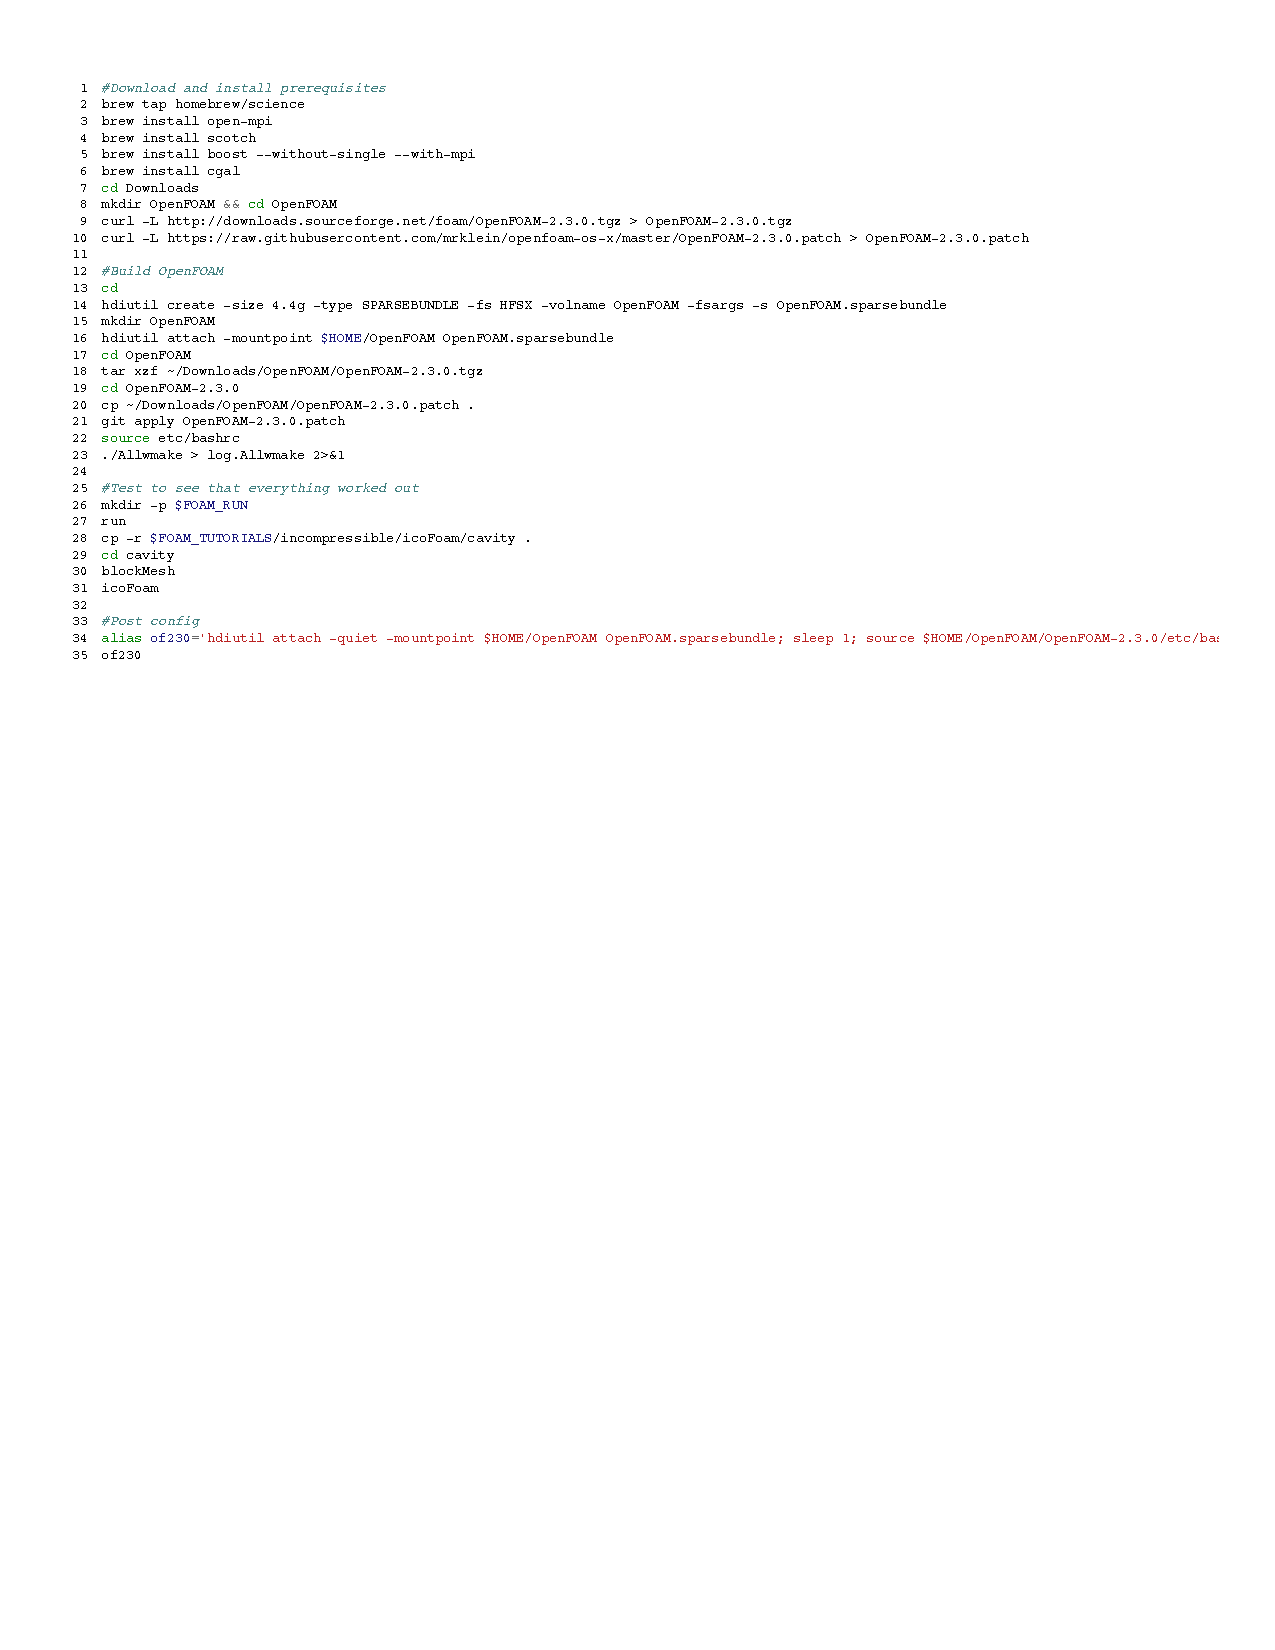
\includegraphics[page=1,width=0.93\textwidth]{of230_install.pdf}
\end{center}
\end{figure}

%%%%%%%%%%%%%%%%%%%%%%%%%%%%%%%%%%%%%%%%%%%%%%%%%%%%%%%%%%%%%%%%%%%%%%
\end{document}
